\documentclass[
	a4paper,
	oneside,
	BCOR = 10mm,
	DIV = 12,
	12pt,
	headings = normal,
]{scrartcl}

%%% Length calculations
\usepackage{calc}
%%%

%%% Support for color
\usepackage{xcolor}
\definecolor{lightblue}{HTML}{03A9F4}
\definecolor{red}{HTML}{F44336}
%%%

%%% Including graphics
\usepackage{graphicx}
%%%

%%% Font selection
\usepackage{fontspec}

\setromanfont{STIX Two Text}[
	SmallCapsFeatures = {LetterSpace = 8},
]

\setsansfont{IBM Plex Sans}[
	Scale = MatchUppercase,
]

\setmonofont{IBM Plex Mono}[
	Scale = MatchUppercase,
]
%%%

%%% Math typesetting
\usepackage{amsmath}

\usepackage{unicode-math}
\setmathfont{STIX Two Math}
%%%

%%% List settings
\usepackage{enumitem}
\setlist[enumerate]{
	label*      = {\arabic*.},
	leftmargin  = *,
	labelindent = \parindent,
	topsep      = 1\baselineskip,
	parsep      = 0\baselineskip,
	itemsep     = 1\baselineskip,
}

\setlist[itemize]{
	label*      = {—},
	leftmargin  = *,
	labelindent = \parindent,
	topsep      = 1\baselineskip,
	parsep      = 0\baselineskip,
	itemsep     = 1\baselineskip,
}

\setlist[description]{
	font        = {\rmfamily\upshape\bfseries},
	topsep      = 1\baselineskip,
	parsep      = 0\baselineskip,
	itemsep     = 0\baselineskip,
}

%%%

%%% Structural elements typesetting
\setkomafont{pagenumber}{\rmfamily}
\setkomafont{disposition}{\rmfamily\bfseries}

% Sectioning
\RedeclareSectionCommand[
	beforeskip = -1\baselineskip,
	afterskip  = 1\baselineskip,
	font       = {\normalsize\bfseries\scshape},
]{section}

\RedeclareSectionCommand[
	beforeskip = -1\baselineskip,
	afterskip  = 1\baselineskip,
	font       = {\normalsize\bfseries\itshape},
]{subsection}

\RedeclareSectionCommand[
	beforeskip = -1\baselineskip,
	afterskip  = 1\baselineskip,
	font       = {\normalsize\bfseries},
]{subsubsection}

\RedeclareSectionCommand[
	beforeskip = -1\baselineskip,
	afterskip  = -0.5em,
	font       = {\normalsize\mdseries\scshape\addfontfeatures{Letters = {UppercaseSmallCaps}}},
]{paragraph}
%%%

%%% Typographic enhancements
\usepackage{microtype}
%%%

%%% Language-specific settings
\usepackage{polyglossia}
\setmainlanguage{ukrainian}
\setotherlanguages{english}
%%%

%%% Captions
\usepackage{caption}
\usepackage{subcaption}

%\DeclareCaptionLabelFormat{closing}{#2)}
%\captionsetup[subtable]{labelformat = closing}

%\captionsetup[subfigure]{labelformat = closing}

\captionsetup[table]{
	aboveskip = 0\baselineskip,
	belowskip = 0\baselineskip,
}

\captionsetup[figure]{
	aboveskip = 1\baselineskip,
	belowskip = 0\baselineskip,
}

\captionsetup[subfigure]{
	labelformat = simple,
	labelformat = brace,
}
%%%

%%% Hyphenated ragged typesetting
\usepackage{ragged2e}
%%%

%%% Table typesetting
\usepackage{booktabs}
\usepackage{longtable}

\usepackage{multirow}

\usepackage{array}
\newcolumntype{v}[1]{>{\RaggedRight\arraybackslash\hspace{0pt}}p{#1}}
\newcolumntype{b}[1]{>{\Centering\arraybackslash\hspace{0pt}}p{#1}}
\newcolumntype{n}[1]{>{\RaggedLeft\arraybackslash\hspace{0pt}}p{#1}}
%%%

%%% Drawing
\usepackage{tikz}
\usepackage{tikzscale}
\usetikzlibrary{positioning}
\usetikzlibrary{arrows.meta} % Stealth arrow tips
%%%

%%% SI units typesetting
\usepackage{siunitx}
\sisetup{
	output-decimal-marker = {,},
	exponent-product      = {\cdot},
	inter-unit-product    = \ensuremath{{} \cdot {}},
	per-mode              = symbol,
}
%%%

%%% Links and hyperreferences
\usepackage{hyperref}
\hypersetup{
	bookmarksnumbered = true,
	colorlinks      = false,
	linkbordercolor = red,
	urlbordercolor  = lightblue,
	pdfborderstyle  = {/S/U/W 1.5},
}
%%%

%%% Length adjustments
% Set baselineskip, default is 14.5 pt
\linespread{1.068966} % ~15.5 pt
\setlength{\emergencystretch}{1em}
\setlength{\parindent}{1.5em}
\newlength{\gridunitwidth}
\setlength{\gridunitwidth}{\textwidth / 12}
%%%

%%% Custom commands
\newcommand{\allcaps}[1]{{\addfontfeatures{LetterSpace = 8, Kerning = Off}#1}}
%%%

\begin{document}

\begin{titlepage}
		\begin{center}
			Міністерство освіти і науки України\\
			Національний авіаційний університет\\
			Навчально-науковий інститут комп'ютерних інформаційних технологій\\
			Кафедра комп'ютеризованих систем управління

			\vspace{\fill}
				Лабораторна робота №3\\
				з дисципліни «Телекомунікаційні~технології комп'ютерних~мереж»\\
				на тему «Оптоволоконні лінії зв'язку»

			\vspace{\fill}

			\begin{flushright}
				Виконав:\\
				студент \allcaps{ННІКІТ}\\
				групи СП-325\\
				Клокун В.\,Д.\\
				Перевірив:\\
				Пушкін Ю.\,О.
			\end{flushright}

			Київ 2018
		\end{center}
	\end{titlepage}

	\section{Мета роботи}
		Ознайомлення з~оптоволоконними засобами комунікації.

	\section{Контрольні запитання}
		\subsection{Структура одномодового волокна}
			Структура типового одномодового волокна~(рис.~\ref{fig:single-mode-fiber-structure}) складається з:
			\begin{enumerate}[noitemsep]
				\item Серцевини (діаметр~— \SI{8}{\micro\metre}), яка переносить світловий промінь.
				\item Оболонки (діаметр~— \SI{125}{\micro\metre}), яка стримує промінь у серцевині за допомогою явища повного внутрішнього відбиття.
				\item Буфера (діаметр~— \SI{250}{\micro\metre}), який механічно ізолює оптичне волокно та~захищає його від~фізичних пошкоджень.
				\item Обшивки (діаметр~— \SI{400}{\micro\metre}), яка забезпечує вторинний захист оптичного волокна та~кабеля в~цілому.
			\end{enumerate}

			\begin{figure}[!htbp]
				\centering
				\def\svgwidth{\columnwidth}
				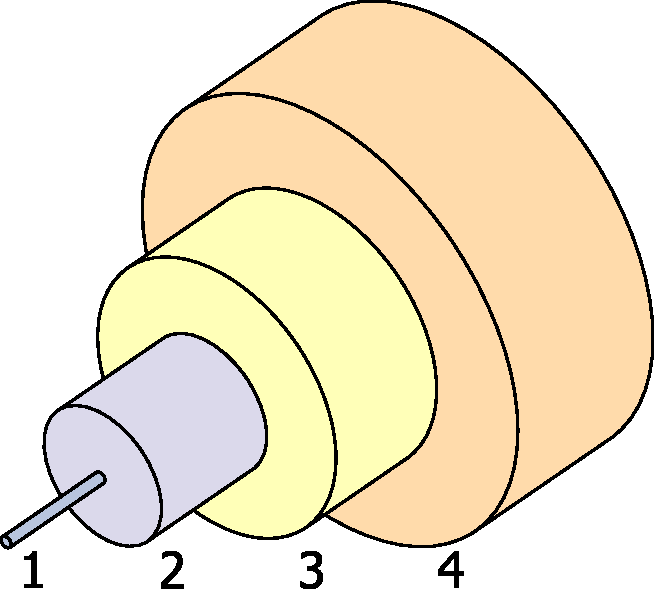
\includegraphics[height = 5\baselineskip]{./assets/single-mode-fiber-structure.pdf}
				\caption{Структура одномодового волокна}
				\label{fig:single-mode-fiber-structure}
			\end{figure}

		\subsection{Що таке коефіцієнт заломлення?}
			Коефіцієнт заломлення~$n$~— це показник, який визначає, у~скільки разів швидкість розповсюдження світла в~середовищі~$v$ менша за~швидкість світла у~вакуумі~$c$:
			\[
				n = \frac{c}{v}.
			\]

		\subsection{Що таке внутрішнє відбиття?}
			Внутрішнє відбиття~(рис.~\ref{fig:internal-reflection-fiber-optical-cable})~— це явище, що~спостерігається при~поширенні хвиль різної оптичної природи в~середовищах, фізичні властивості яких змінюються в~просторі. Це явище використовується у~волоконно-оптичних кабелях для~утримання світлового випромінювання у~межах серцевини кабеля.

			\begin{figure}[!htbp]
				\centering
				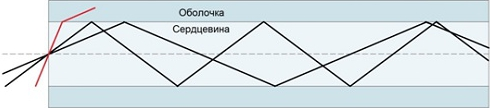
\includegraphics[height = 4\baselineskip]{./assets/total-internal-reflection.jpg}
				\caption{Внутрішнє відбиття у~волоконно-оптичному кабелі}
				\label{fig:internal-reflection-fiber-optical-cable}
			\end{figure}

			Повне внутрішнє відбиття спостерігається тоді, коли поширювана хвиля падає на~межу двох середовищ під~кутом, більшим за~певний критичний кут, відносно нормалі. Якщо середовище, що~знаходиться за~межею, має менший показник заломлення, і~кут падіння більший за~критичний кут, хвиля не~може перетнути межу і~повністю відбивається.

		\subsection{Які Ви знаєте типи волокон?}
			Існують такі типи волокон:
			\begin{enumerate}[noitemsep]
				\item Одномодове.
				\item Багатомодове.
				\item Градієнтне~— у такому волокні коефіцієнт заломлення у серцевині зменшується поступово від осі до зовнішньої стинки волокна, що змушує промені світла вигинатись дугою при наближенні до оболонки, на відміну від відбиття на межі розділу компонентів волокна.
				\item Поляризаційно-стабільне~— волокно, що утримує існуючу поляризацію лінійно поляризованого світлового променя, введеного у волокно за умови правильної орієнтацію.
				\item Фотонно-кристалічне~— волокно, світловоди якого працюють завдяки властивостям фотонних кристалів.
			\end{enumerate}

		\subsection{Розповсюдження світлових променів через багатомодові оптичні світловоди}
			\begin{figure}[!htbp]
				\centering
				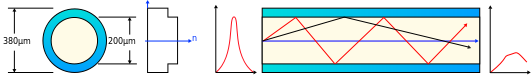
\includegraphics[height = 4\baselineskip]{./assets/fibre-multimode.png}
				\caption{Розповсюдження світлових променів через багатомодовий оптичний світловод: діаметри кабеля, коефіцієнти заломлення, вхідний імпульс, шлях променів та~вихідний імпульс}
			\end{figure}

		\subsection{Що таке загасання і його причини?}
			Загасання~— це~зменшення інтенсивності світлових променів у~волокнах відносно подоланої ними відстані у~середовищі передачі. Причинами загасання є~розсіювання світла та~інфрачервоне і~ультрафіолетове поглинання.

		\subsection{Що таке дифузне відбиття світла?}
			Дифузне відбиття світла~(рис.~\ref{fig:diffuse-reflection})~— це явище, при якому відбивання світлових променів відбувається під кутом, відмінним від кута падіння.

			\begin{figure}[!htbp]
				\centering
				\begin{subfigure}{0.5\textwidth}
					\centering
					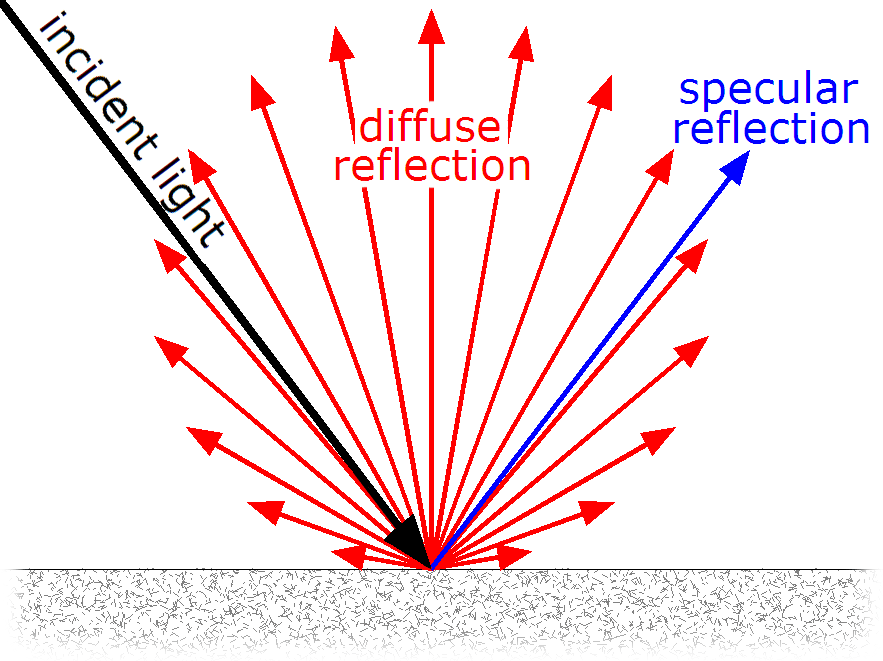
\includegraphics[height = 8\baselineskip]{./assets/diffuse-reflection-lambert.png}
					\caption{}
					\label{subfig:diffuse-reflection-labertian}
				\end{subfigure}%
				\begin{subfigure}{0.5\textwidth}
					\centering
					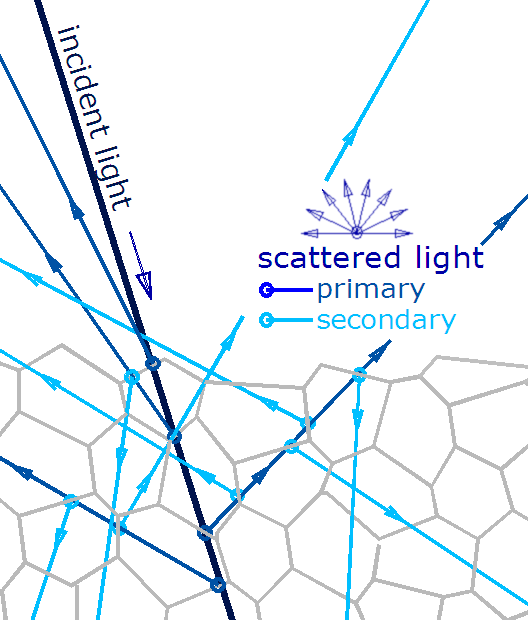
\includegraphics[height = 8\baselineskip]{./assets/diffuse-reflection-subsurface.png}
					\caption{}
					\label{subfig:diffuse-reflection-subsurface}
				\end{subfigure}
				\caption{Дифузійне відбиття світла}
				\label{fig:diffuse-reflection}
			\end{figure}

			В~загальному випадку дифузне відбиття світла викликане не~нерівністю поверхні, а~підповерхневими центрами заломленнями.

		\subsection{Ультрафіолетове та інфрачервоне поглинання}
			Ультрафіолетове та~інфрачервоне поглинання є~однією з~причин загасань у~волоконно-оптичному кабелі. Причиною поглинання в~ультрафіолетовому діапазоні є~резонанс електронних оболонок матеріалу; причиною поглинання в~інфрачервоному діапазоні є~резонанс атомів кремнію як~системи: деяка складова загальної спектральної смуги світла збігається з~частотою коливань елементів кристалічної решітки чи~молекулярної структури тіла.

		\subsection{Що таке чіпкування та зрощення?}
			Оптичні кабелі можуть бути з'єднані один із одним за допомогою спеціальних роз'ємів або зрощення, що у кінцевому результаті створює безперервний оптичний хвилевід. Зрощення~— це процес створення нероз'ємних з'єднань оптичних волокон. Загальноприйнятим методом зрощення є дугове зварювання, при якому кінці волокон нагріваються електричною дугою та з'єднуються.

			Чіпкування~— це процес термінації, тобто додавання конекторів у~кінці кабеля, які~точно і~надійно закріплюють кінець оптичного волокна. Волоконно-оптичний конектор~— це твердий циліндр, оточений муфтою, яка~тримає циліндр у~роз'ємі. Встановлення конектора зазвичай виконується так: кінець оптичного волокна готують до~приєднання та~вставляють в~задню частину конектора; зазвичай для~надійного закріплення волокна використовується швидкозастигаючий клей, та~до~задньої сторони конектора під'єднується компенсатор механічного навантаження. Після застигання клею, кінець оптичного волокна полірується до~дзеркального вигляду, в~залежності від~застосування використовуються різні види полірування: для~одномодових кабелів кінці оптичного волокна зазвичай полірують з~невеликим вигином, завдяки якому з'єднані конектори торкаються лише серцевинами.

		\subsection{Застосування оптоволокна}
			Найширше оптичне волокно застосовується для організації зв'язку та~у~датчиках. Використання оптичних волокон для~ліній зв'язку обумовлене тим, що~воно забезпечує високу захищеність від~несанкціонованого доступу, низьке загасання сигналу при~передачі на~великі відстані, можливість передачі інформації з~надвисокими швидкостями та~пропускною здатністю.

			Оптоволоконна система передачі даних складається з~3~основних компонентів: джерела світла, носія світлового сигналу та~приймача сигналу (детектора). Під'єднавши до~одного кінця оптичного волокна джерело світла, а~до~іншого~— детектор, ми отримаємо однонаправлену систему передачі даних: світло поширюється в~надтонкому скляному волокні, при~попаданні світла на~детектор генерується електричний імпульс. Світловий імпульс приймають за~одиницю, а~відсутність імпульсу~— за~нуль.

			Оптичне волокно може бути використане як~датчик для~вимірювання напруги, температури та~інших параметрів. Невеликий розмір та~фактична відсутність необхідності в~електричній енергії надають волоконно-оптичним датчикам перевагу перед традиційними електричними у~деяких областях. Оптичне волокно використовується у~гідрофонах у~сейсмічних чи~гідролокаційних пристроях, а~також у~лазерних мікрофонах, гіроскопах та~інших пристроях.

			Оптоволокно широко використовується для освітлення. Наприклад, як світлопроводи в медичних, декоративних та інших цілях, для формування зображення та організації ліній зв'язку.

	\section{Висновок}
		Виконуючи дану лабораторну роботу, ми ознайомились з~оптоволоконними засобами комунікації.

\end{document}
